
In what follows I make a quick inventory of the main codes of computational geodynamics, 
for crust, lithosphere and/or mantle modelling.
In order to find all CIG-codes citations go to: 
\url{https://geodynamics.org/cig/news/publications-refbase/}

\begin{itemize}

%------------------------------------------------------------------------------
\item {\codefont ABAQUS} \index{general}{ABAQUS code}
%------------------------------------------------------------------------------

\begin{scriptsize}
\begin{itemize}
\item[\nineteeneightyeight]  \textcite{reyu98}
\item[\twothousand]          \textcite{reyu00}
\item[\twothousandone]       \textcite{brry01}
\item[\twothousandtwo]       \textcite{gedh02}
\item[\twothousandthree]     \textcite{fumr03}
\item[\twothousandsix]       \textcite{hapf06}
\item[\twothousandseven]     \textcite{camg07}
\item[\twothousandnine]      \textcite{kuhe09}, \textcite{makh09}
\item[\twothousandten]       \textcite{camg10}
\item[\twothousandtwelve]    \textcite{nalr12}
\item[\twothousandthirteen]  \textcite{soyl13}
\item[\twothousandfifteen]   \textcite{pevp15}
\item[\twothousandseventeen] \textcite{naam17}
\item[\twothousandeighteen]  \textcite{naam18}
\end{itemize}
\end{scriptsize}

%------------------------------------------------------------------------------
\item {\codefont ACuTEMan} \index{general}{ACuTEMan code}
%------------------------------------------------------------------------------
A multigrid-based mantle convection simulation code

\begin{scriptsize}
\begin{itemize}
\item[\twothousandfive] Kameyama \cite{kame05}, Kameyama \etal \cite{kaks05}
\item[\twothousandfifteen] Miyagoshi \etal \cite{miko15}, Kameyama \etal \cite{kamo15}
\item[\twothousandtwenty] Miyagoshi \etal \cite{miko20} 
\end{itemize}
\end{scriptsize}

%------------------------------------------------------------------------------
\item {\codefont ANSYS} \index{general}{ANSYS code}
%------------------------------------------------------------------------------

\begin{scriptsize}
\begin{itemize}
\item Nem{\v{c}}ok \& Henk \cite{nehe06}
\item Guo \etal \cite{guyr16}
\end{itemize}
\end{scriptsize}

%------------------------------------------------------------------------------
\item {\codefont ADELI} \index{general}{ADELI code}
%------------------------------------------------------------------------------

Belonging to the same family as the FLAC 
(Fast Lagrangian Analysis of Continua; Cundall and Board, 1988 \cite{cubo88}) 
and Parovoz codes 
(Poliakov and Podladchikov, 1992 \cite{popo92}; Gerbault \etal, 2009 \cite{gecm09}), 
ADELI is based on an explicit temporal
finite difference approach associated with the dynamic relaxation method (Underwood, 1983). 
Numerical and mechanical aspects of this code in a 2-D or 3-D context can be 
found in Hassani \etal (1997) \cite{hajc97} and Ch\'ery \etal (2001) \cite{chzh01}.

\url{https://code.google.com/archive/p/adeli/}

\url{https://code.google.com/archive/p/adeli/wikis/Publications.wiki}

\begin{scriptsize}
\begin{itemize}
\item[\nineteenninetysix] Hassani \& Ch\'ery \cite{hach96b}
\item[\nineteenninetyseven] Hassani \etal\cite{hajc97}
\item[\nineteenninetyeight] Huc \etal \cite{huhc98}
\item[\nineteenninetynine] Vanbrabant \etal \cite{vajh99}
\item[\twothousand] Lesne \etal \cite{lecd00}
\item[\twothousandone] Ch\'ery \etal \cite{chzh01}
\item[\twothousandthree] Provost \etal \cite{prch03}
\item[\twothousandfour] Godard \etal \cite{gocl04}, Berger \etal \cite{bejh04}
\item[\twothousandsix] Vernant \& Chery \cite{vech06}, Godard \etal \cite{golc06}
\item[\twothousandeight] Bonnardot \etal \cite{boht08a,boht08b}, Got \etal \cite{gomm08},
                         Neves \etal \cite{netv08}
\item[\twothousandtwelve] Gerbault \etal \cite{gech12}, Gibert \etal \cite{gigh12}
\item[\twothousandthirteen] Wang \etal \cite{wahd13}
\item[\twothousandfourteen] Cerpa \etal \cite{cehg14}, Messager \etal \cite{mehn14}
\item[\twothousandfifteen] Cerpa \etal \cite{ceag15}
\item[\twothousandeighteen] Cerpa \etal \cite{cegm18}, Gerbault \etal \cite{gehn18}
\item[\twothousandnineteen] Tarayoun \etal \cite{tamg19}
\end{itemize}
\end{scriptsize}

%------------------------------------------------------------------------------
\item \aspect \index{general}{ASPECT code}
%------------------------------------------------------------------------------

This code is hosted by CIG at \url{https://geodynamics.org/cig/software/aspect/}. 
It is an open source community code based on the finite element library deal.II \cite{bahk07,arbc19,arbd20}. 
It is massively parallel, relies on the p4est library for adaptive mesh refinement,
uses the Trilinos solver library \cite{hewi12}, and can deal with 2D and 3D geometries. 

\begin{scriptsize}
\begin{itemize}
\item[\twothousandtwelve] Kronbichler \etal \cite{krhb12}
\item[\twothousandfifteen] Austermann \etal \cite{aupm15}, Tosi \etal \cite{tosn15}
\item[\twothousandsixteen] Dannberg \& Heister \cite{dahe16}, Gassmoeller \etal \cite{gadb16}, 
                           Zhang \& O'Neill \cite{zhon16}
\item[\twothousandseventeen] He \etal \cite{hepb17}, Dannberg \etal \cite{daef17}, 
                             Heister \etal \cite{hedg17}, Rose \etal \cite{robh17}, 
                             Rose \& Buffett \cite{robu17}, Austermann \etal \cite{aumh17},
                             Thieulot \cite{thie17}, Bredow \etal \cite{brsg17}, 
                             O'Neill \etal \cite{onmz17}, Takeyama \etal \cite{tasm17}
\item[\twothousandeighteen] Dannberg \& Gassmoeller \cite{daga18}, O'neill \& Zhang \cite{onzh18}, 
                            Glerum \etal \cite{gltf18}
                            Gassmoeller \etal \cite{galh18}, 
                            Perry-Houts \& Karlstrom \cite{peka18}, Puckett \etal \cite{puth18},
                            Bredow \& Steinberger \cite{brst18b}, Zhang \& Li \cite{zhli18}
\item[\twothousandnineteen] Bauville \& Baumann \cite{baba19}, Steinberger \etal \cite{stbl19}, 
                            Corti \etal \cite{cocf19}, Liu \& King \cite{liki19}, 
                            Gassmoeller \etal \cite{galb19}, Dannberg \etal \cite{dagg19},
                            Njinju \etal \cite{njas19}, \textcite{sepg19}, 
                            Robey \etal \cite{ropu19}, Fraters \etal \cite{frtv19,frbt19},
                            Lin \etal \cite{lixs19}, \textcite{hepm19}, Heron \etal \cite{heps19}, 
                            \textcite{perr19}
\item[\twothousandtwenty] Gassmoeller \etal \cite{gadb20}, Farangitakis \etal \cite{fahm20}, 
                          Louis-Napoleon \etal \cite{logb20}, Heyn \etal \cite{hect20,hect20b}, 
                          Glerum \etal \cite{glbs20}
                          Naliboff \etal \cite{nagb20}, Citron \etal \cite{cilw20},
                          Heron \etal \cite{hemn20}, O'Neill \etal \cite{onlw20}, 
                          Assanelli \etal \cite{aslr20}, Muluneh \etal \cite{mubi20},
                          Negredo \etal \cite{nemc20}, Lesher \etal \cite{ledb20},
                          Mitrovica \etal \cite{miac20}, Withers \cite{with20},
                          Lees \etal \cite{lerm20}
\item[\twothousandtwentyone] \textcite{balm21}, \textcite{brst21},
                             \textcite{sacp21}, \textcite{grrm21},
                             \textcite{hebg21}, \textcite{njsn21}, 
                             \textcite{clhe21}, \textcite{fabh21},
                             \textcite{nebg21}, \textcite{cosb21},
                             \textcite{gona21}, \textcite{sabg21},
                             \textcite{hoco21}, \textcite{frbi21},
                             \textcite{manp21}, \textcite{sepg21},
                             \textcite{thba21}
\end{itemize}
\end{scriptsize}

%------------------------------------------------------------------------------
\item {\codefont BASIL \& ELLE} 
%------------------------------------------------------------------------------

From \url{http://homepages.see.leeds.ac.uk/~eargah/basil/}:
Basil is a finite element program which calculates quantities which describe  stress  and strain in non-linear viscous materials, for strains up to the of order 100\%.   
The calculations  describe  very  viscous  Earth materials which undergo irreversible large-strain 
deformation at  high  temperature  and over long time periods, under the influence of body 
forces and surface tractions.  Sybil  is the post-processing program that permits basil 
solutions to be examined in detail using an interactive graphical user interface.

The program permits a spatially variable Newtonian  or  non-Newtonian  viscosity  in a 2-D 
geometry with boundary conditions on traction and/or velocity.  It is also  possible  
to include  a single fault or discontinuity in the problem in a dynamically self consistent way.  
The 2-D deformation  field represents  either plane-strain deformation, or it permits 
a specified distribution of normal stress in the third  direction.   The  latter is referred 
to as the thin viscous sheet formulation when the normal force is due to  gravity  acting on 
variations of the layer thickness.  Plane-stress calculations are a specific case of 
the thin viscous sheet formulation.

The programs basil and sybil have been developed  mainly  at Monash  University  since  1988,  
and before that at ANU and Harvard.  The present set of  programs  has  been  developed mainly  by  
Greg  Houseman, Terence  Barr  and  Lynn Evans.

ELLE is an open-source multi-process and multi-scale software for the simulation of geologic processes, especially (but not only) during deformation and metamorphism. It is coupled to/based on BASIL. See \url{http://elle.ws/} for a complete list of publications.

\begin{scriptsize}
\begin{itemize}
\item[\nineteenninetytwo] Barr \& Houseman \cite{baho92}(?)
\item[\nineteenninetysix] Barr \& Houseman \cite{baho96}, Houseman \& England \cite{hoen96}
\item[\nineteenninetyseven] Houseman \& Gubbins \cite{hogu97}, Houseman \& Molnar \cite{homo97},
                            Bons \etal \cite{bobt97}, Neil \& Houseman \cite{neho97}
\item[\twothousand] Houseman \etal \cite{honk00}
\item[\twothousandone] Tenczer \etal \cite{tesb01}
\item[\twothousandeight] Bons \etal \cite{bokj08}
\item[\twothousandnineteen] Llorens \cite{llor19}
\end{itemize}
\end{scriptsize}

%------------------------------------------------------------------------------
\item {\codefont BEM} 
\index{general}{Fast Multipole-accelerated Boundary Element Method} 
\index{general}{Boundary Element Method} 
\index{general}{BEM} 
%------------------------------------------------------------------------------

\begin{scriptsize}
\cite{crsr83}\\
Katzman \etal \cite{katl95}\\
Morra \etal \cite{moct07}\\
Morra \etal \cite{moct09}\\
Morra \etal \cite{moyb10}\\
Quevedo \etal \cite{qumm12}, Butterworth \etal \cite{buqm12}, Li \& Ribe \cite{liri12}\\
Quevedo \etal \cite{quhm13}\\
Di Leo \etal \cite{diwl14}, Li \etal \cite{lidr14}\\
Xu \& Ribe \cite{xuri16}\\
Gerardi \etal \cite{gert19}
\end{scriptsize}

%------------------------------------------------------------------------------
\item {\codefont CHIC}  \index{general}{CHIC code}
%------------------------------------------------------------------------------

\begin{scriptsize}
\textcite{norv15}
\end{scriptsize}

%------------------------------------------------------------------------------
\item \citcoms and {\codefont CitComCU} \index{general}{CitComS code}
%------------------------------------------------------------------------------

Citcom (California Institute of Technology COnvection in the Mantle) was  developed by Louis
Moresi at the California Institute of Technology (Moresi, 1992). This code solved the equations
of viscous fluid dynamics, and, as the name implies, was geared towards modelling convection in
the Earth's mantle. Moresi and Solomatov (\nineteenninetyfive) provide a detailed description of the multigrid
finite element algorithm. After this and during his time at CSIRO, Dr. Moresi modified the code to
include mobile integration points. The code became a particle-in-cell finite-element code named
CIItcom , which was able to track and evolve material properties on particles. This work at
CSIRO resulted in a new generation of the software, named Ellipsis.

\begin{center}
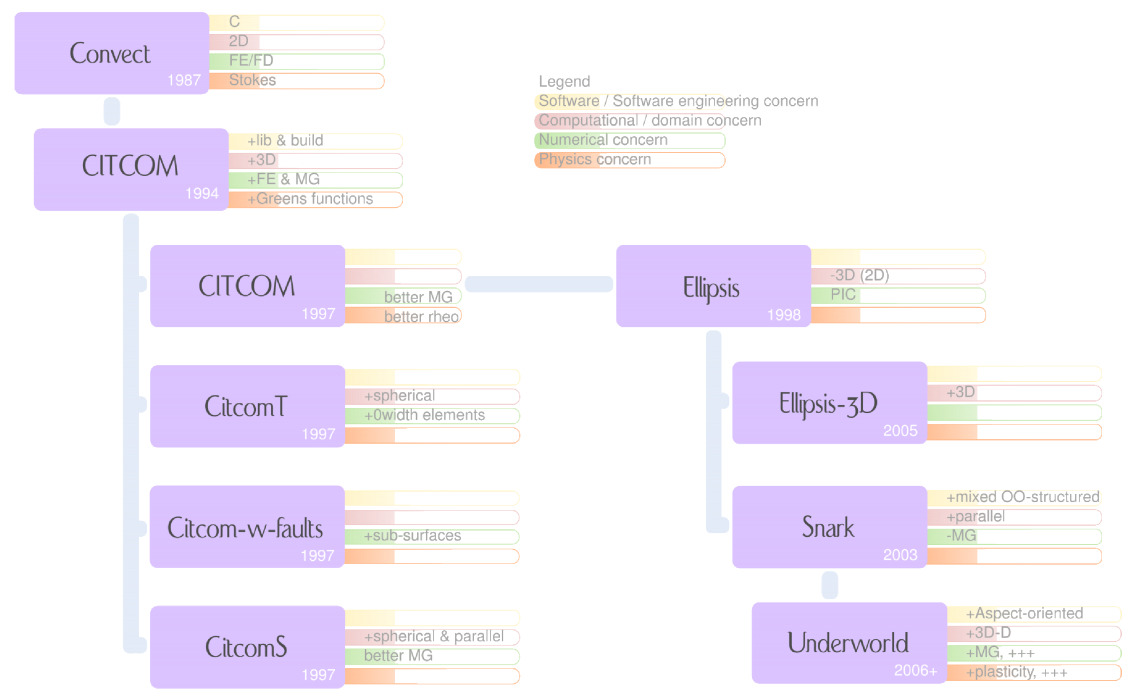
\includegraphics[width=10cm]{images/codes/quenette_cig_2009}\\
{\captionfont Taken from a presentation give by Quenette at CIG meeting in 2009.}
\end{center}

\begin{center}
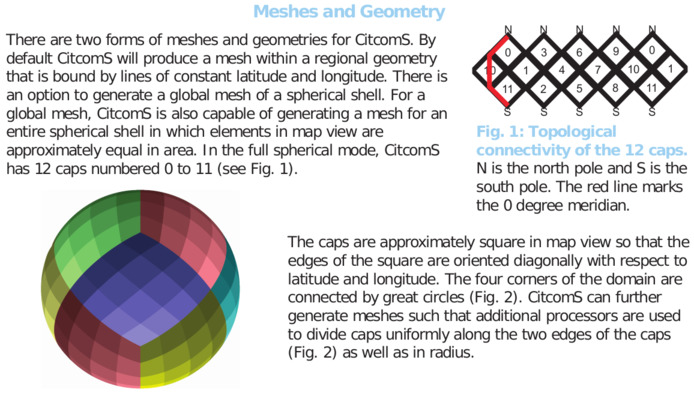
\includegraphics[width=8cm]{images/codes/CitcomS}\\
{\captionfont Taken from a poster by Tan \etal at Geomath, Sept. 26th, 2008.}
\end{center}

These codes are hosted by CIG at\\
\url{https://geodynamics.org/cig/software/citcomcu/}  \\
\url{https://geodynamics.org/cig/software/citcoms/}

\begin{scriptsize}
\begin{itemize}
\item[\nineteenninetyfive] Moresi \& Solomatov \cite{moso95}, Moresi \& Parsons \cite{mopa95}
\item[\nineteenninetysix] Solomatov \& Moresi \cite{somo96}, Moresi \& Gurnis \cite{mogu96}, 
                    Zhong \& Gurnis \cite{zhgu96}
\item[\nineteenninetyseven] Moresi \& Lenardic \cite{mole97}, Burgess \etal \cite{bugm97}, 
                    Solomatov \& Moresi \cite{somo97}
\item[\nineteenninetyeight] Moresi \& Solomatov \cite{moso98}, Zhong \etal \cite{zhgm98}, 
                    Gurnis \etal \cite{gumm98}, Reese \etal \cite{resm98}
\item[\nineteenninetynine] Moresi \& Lenardic \cite{mole99}, Burgess \& Moresi \cite{bumo99}, 
                    van Keken \& Zhong \cite{vazh99}, Lenardic \& Moresi \cite{lemo99}, 
                    Reese \etal \cite{resm99}
\item[\twothousand] Zhong \etal \cite{zhzm00}, Gurnis \etal \cite{gumr00,gumm00},
                    Lenardic \etal \cite{lemm00}, Solomatov \& Moresi \cite{somo00}
\item[\twothousandone] Billen \& Gurnis \cite{bigu01}, Lenardic \& Moresi \cite{lemo01},
                    Zhong \cite{zhon01}
\item[\twothousandtwo] Tan \etal \cite{tagh02}, Solomatov \& Moresi \cite{somo02}
\item[\twothousandthree] van Hunen \& Zhong \cite{vazh03}, Conrad \& Gurnis \cite{cogu03},
                    Billen \& Gurnis \cite{bigu03}, Lenardic \etal \cite{lemm03},
                    Lenardic \& Moresi \cite{lemo03}, Billen \etal \cite{bigs03}, 
                    Vezolainen \etal \cite{vesh03}
\item[\twothousandfour] Ke \& Solomatov \cite{keso04}, Solomatov \cite{solo04},
                    Freeman \etal \cite{frmm04}, Lenardic \etal \cite{lenm04},
                    Cooper \etal \cite{colm04}, McNamara \etal \cite{mczh04}, 
                    Vezolainen \etal \cite{vesb04}, Roberts \& Zhong \cite{rozh04}
\item[\twothousandfive] van Hunen \etal \cite{vazs05}, Billen \& Hirth \cite{bihi05},
                    McNamara \& Zhong \cite{mczh05a}\cite{mczh05b},
                    Lenardic \etal \cite{lemj05}, Zhong \cite{zhon05}
\item[\twothousandsix] Solomatov \& Barr \cite{soba06}, Becker \cite{beck06}
                    Piromallo \etal \cite{pibf06}, Tan \etal \cite{tact06},
                    Becker \etal \cite{besb06}, Conrad \& Lithgow-Bertelloni \cite{coli06},
                    Freeman \etal \cite{frmm06}, Cooper \etal \cite{colm06},
                    Zhong \cite{zhon06}, Ke \& Solomatov \cite{keso06},
                    Roberts \& Zhong \cite{rozh06}, Zhang \& Pysklywec \cite{zhpy06}
\item[\twothousandseven] Solomatov \& Barr \cite{soba07}, Billen \& Hirth \cite{bihi07},
                   Zhong \etal \cite{zhzl07}, Manea \& Gurnis \cite{magu07},
                   Ballmer \etal \cite{bavi07}, Ritsema \etal \cite{rimb07},
                   Moucha \etal \cite{mofm07}, Conrad \etal \cite{cobs07},
                   Quenette \etal \cite{qums07}, Huang \& Davies \cite{huda07},
                   Roberts \& Zhong \cite{rozh07}
\item[\twothousandeight] \cite{gamc08},
                    Zhong \etal \cite{zhmt08}, Hoink \& Lenardic \cite{hole08},
                    Lenardic \etal \cite{lejm08}, Liu \etal \cite{lisg08},
                    Chen \etal \cite{chzy08}, Becker \etal \cite{beke08},
                    Becker \cite{beck08}, Sleep \cite{slee08},
                    Leng \& Zhong \cite{lezh08}, King \cite{king08},
                    Liu \& Gurnis \cite{ligu08}, Metivier \& Conrad \cite{meco08},
                    Roberts \& Nimmo \cite{roni08}, Spasojevic \etal \cite{splg08},
                    Di Giuseppe \etal \cite{divf08}, van Wijk \etal \cite{vavg08}
\item[\twothousandnine] Ke \& Solomatov \cite{keso09}, Bull \etal \cite{bumr09}, 
                    Li \& Zhong \cite{lizh09}, Armitage \etal \cite{arhm09},
                    Zhang \etal \cite{zhzm09}, Andrews \& Billen \cite{anbi09},
                    Foley \& Becker \cite{fobe09}, Burkett \& Billen \cite{bubi09},
                    Becker \& Faccenna \cite{befa09}, Ballmer \etal \cite{bavi09},
                    Leng \& Zhong \cite{lezh09}, Bower \etal \cite{bogj09},
                    Zhong \cite{zhon09}, Conrad \& Husson \cite{cohu09},
                    Cooper \& Conrad \cite{coco09}, Manea \etal \cite{maml09},
                    Naliboff \etal \cite{nacl09}, Roberts \etal \cite{rolm09},
                    Spasojevic \etal \cite{splg09}
\item[\twothousandten] Leng \& Zhong \cite{lezh10}, Bull \etal \cite{bumb10}, 
                 van Wijk \etal \cite{vabv10}, Ballmer \etal  \cite{baiv10},
                 Burkett \& Billen \cite{bubi10}, Zhang \etal \cite{zhzl10},
                 Billen \cite{bill10}, Conrad \& Behn \cite{cobe10},
                 Jadamec \& Billen \cite{jabi10}, Zhu \etal \cite{zhst10},
                 Boschi \etal \cite{bofb10}, Hoink \& Lenardic \cite{hole10},
                 Harig \etal \cite{hazs10}, Faccenna \cite{fabl10},
                 DiCaprio \etal \cite{dimg10}, Faccenna \& Becker \cite{fabe10},
                 Ghosh \etal \cite{ghbz10}, Lassak \etal \cite{lamg10},
                 McNamara \etal \cite{mcgr10}, Shepard \etal \cite{shml10},
                 Spasojevic \etal \cite{spgs10a,spgs10b}, Sramek \& Zhong \cite{srzh10}
\item[\twothousandeleven] Becker \& Faccenna \cite{befa11}, Lenardic \etal \cite{lemj11},
                    van Hunen \& Allen \cite{vaal11}, Leng \& Gurnis \cite{legu11},
                    Liu \& Stegman \cite{list11}, Ballmer \etal \cite{baiv11},
                    Bower \etal \cite{bowg11}, Trubitsyn \etal \cite{tree11},
                    Obermaier \etal \cite{obbh11}, Bianco \etal \cite{bics11}, 
                    Zhang \etal \cite{zhxy11}, Di Caprio \cite{digm11}, 
                    Orth \& Solomatov \cite{orso11}, Matthews \etal \cite{mahg11},
                    Tan \etal \cite{talz11}, Ramsay \& Pysklywec \cite{rapy11},
                    Schaefer \etal \cite{scbb11}, van Hinsbergen \cite{vasd11},
                    van Summeren \etal \cite{vacg11}, Zhang \& Zhong \cite{zhzh11}
\item[\twothousandtwelve] Arredondo \& Billen \cite{arbi12}, Jadamec \& Billen \cite{jabi12},
                    Billen \& Jadamec \cite{bija12}, Bottrill \etal \cite{bova12},
                    Husson \etal \cite{hucf12}, Zhong \etal \cite{zhym12},
                    Hines \& Billen \cite{hibi12}, Jadamec \etal \cite{jabk12},
                    Manea \etal \cite{mapm12}, Solomatov \cite{solo12}, 
                    Trubitsyn \cite{trub12}, Cottaar \& Buffett \cite{cobu12},
                    Han \etal \cite{hats12}, Hoink \etal \cite{holr12},
                    Husson \& Conrad \cite{huco12}, Liu \& Stegman \cite{list12},
                    Miller \& Becker \cite{mibe12}, van Summeren \etal \cite{vacl12},
                    Natarov \& Conrad \cite{naco12}, Roberts \& Arkani-Hamed \cite{roar12},
                    Roberts \& Barnouin \cite{roba12}, Shepard \etal \cite{shlm12},
                    Sramek \& Zhong \cite{srzh12}, Weller \& Lenardic \cite{wele12},
                    Zhang \etal \cite{zhzf12}, \cite{zams12},
                    Magni \etal \cite{mavf12}
\item[\twothousandthirteen] Ballmer \etal \cite{bacs13}, Bower \etal \cite{bogs13a,bogs13b},
                            Jadamec \etal \cite{jabr13}, Quere \etal \cite{qula13},
                            Olson \etal \cite{oldh13}, Arrial \& Billen \cite{arbi13},
                            Conrad \etal \cite{cost13}, Burkett \& Gurnis \cite{bugu13},
                            Flament \etal \cite{flgm13}, Conrad \cite{conr13},
                            Ghosh \etal \cite{ghbh13}, Huang \etal \cite{huyz13},
                            Key \etal \cite{kecl13}, van Summeren \etal \cite{vagc13},
                            Magni \etal \cite{mafv13}, Alpert \etal \cite{almb13}
\item[\twothousandfourteen] Rudolph \& Zhong \cite{ruzh14}, \cite{flgw14}
                            Bull \etal \cite{budt14}, Kaislaniemi \& van Hunen \cite{kava14},
                            Arrial \etal \cite{arfw14}, Wang \etal \cite{wavp14},
                            Sekhar \& King \cite{seki14}, Agrusta \etal \cite{agvg14},
                            Magni \etal \cite{mabv14}, Zhu \cite{zhu14}
\item[\twothousandfifteen] Wong \& Solomatov \cite{woso15}, Zhong \& Rudolph \cite{zhru15}, 
                    Ballmer \etal \cite{bacs15}, Bower \etal \cite{bogf15},
                    Bouilhol \etal \cite{bomv15}, Seton \etal \cite{sefw15},
                    Dannberg \& Sobolev \cite{daso15}, van Hunen \& Miller \cite{vami15},
                    Wang \etal \cite{wazh15}, Wang \etal \cite{wavp15},
                    Wang \etal \cite{waav15}, Hassan \etal \cite{hafg15},
                    Leng \& Gurnis \cite{legu15}, Taramon \etal \cite{tarn15}, 
                    King \cite{king15},
                    Ballmer \etal \cite{basn15}, Motoki \& Ballmer \cite{moba15},
                    Liu \& Zhong \cite{lizh15}, Weller \etal \cite{welo15},
                    Williams \etal \cite{wilm15}, Wang \etal \cite{wahz15},
                    Holt \etal \cite{hobb15}
\item[\twothousandsixteen] Wong \& Solomatov \cite{woso16a,woso16b}, Weller \etal \cite{welm16},
                    Weller \& Lenardic \cite{wele16}, Jadamec \cite{jada16,jada16b},
                    Fritzell \etal \cite{frbs16}, Rodriguez-Gonzalez \etal \cite{robn16},
                    Bobrov \& Baranov \cite{boba16}, Maunder \etal \cite{mavm16},
                    Gu \etal \cite{gulm16}, Kiefer \& Li \cite{kili16},
                    McKinnon \etal \cite{mcnw16}, Wang \etal \cite{wahz16},
                    Yang \& gurnis \cite{yagu16}, Hu \etal \cite{hulh16}
\item[\twothousandseventeen] Agrusta \etal \cite{aggv17}, Magni \etal \cite{maav17},
                       Freeburn \etal \cite{frbm17}, Haynie \& Jadamec \cite{haja17},
                       MacDougall \etal \cite{majf17}, Ghosh \etal \cite{ghts17},
                       Taposeea \etal \cite{taac17}, Yang \etal \cite{yagz17},
                       Li \& Zhong \cite{lizh17}, Holt \& Becker \cite{hobe17},
                       Zhou \& Liu \cite{zhli17}
\item[\twothousandeighteen] Heyn \etal \cite{hect18}, King \cite{king18},
                    Kaislaniemi \etal \cite{kavb18}, Wang \etal \cite{wavp18},
                    Hu \etal \cite{hulz18}, Li \etal \cite{lizo18},
                    Citron \etal \cite{cimt18}, Trubitsyn \& Evseev \cite{trev18},
                    Weller \& Lenardic \cite{wele18}, Yang \etal \cite{yagz18},
                    Mao \& Zhong \cite{mazh18}, Billen \& Arredondo \cite{biar18},
                    Li \& Zhong \cite{lizh19}
\item[\twothousandnineteen] Flament \cite{flam19}, Maunder \etal \cite{mavb19},
                    Fuchs \& Becker \cite{fube19}, Magni \cite{magn19}, 
                    Ma \etal \cite{malg19}, Mao \& Zhong \cite{mazh19},
                    Bobrov \& Baranov \cite{boba19}, Lenardic \etal \cite{lewh19},
                    Schliffke \etal \cite{scvm19}, Allu Peddinti \& McNamara \cite{almc19},
                    Reali \etal \cite{rejv19}, Huang \etal \cite{huzl19},
                    Paul \etal \cite{pagc19}
\item[\twothousandtwenty]    \textcite{weki20},  \textcite{braf20},  \textcite{pagh20},
                             \textcite{vamg20},  \textcite{heyg20},  \textcite{loru20}, 
                             \textcite{bill20},  \textcite{sele20},
                             \textcite{dazl20},  \textcite{wali20}, 
\item[\twothousandtwentyone] \textcite{cafm21},  \textcite{ligl21},
                             \textcite{scvg21},  \textcite{ligl21b},
                             \textcite{wali21},  \textcite{cafb21}
\item[\twothousandtwentytwo] \textcite{limc22} 
\end{itemize}
\end{scriptsize}


%------------------------------------------------------------------------------
\item {\codefont COMSOL} \index{general}{COMSOL}
%------------------------------------------------------------------------------

\begin{scriptsize}
\twothousandeight
\textcite{vack08}
\twothousandtwelve
\textcite{ronb12}
\twothousandfourteen
\textcite{cuwi14}
\textcite{paml14b}
\twothousandfifteen
\textcite{rasg15},
\textcite{khfh15}
\twothousandtwentyone
\textcite{chap21},
\textcite{trbs21},
\textcite{khmo21}
\end{scriptsize}

%------------------------------------------------------------------------------
\item {\codefont ConMan} \index{general}{ConMan code}\index{general}{SCAM code}
%------------------------------------------------------------------------------
This code is hosted by CIG at \url{https://geodynamics.org/cig/software/conman/}

\begin{scriptsize}
\begin{itemize}
\item[\nineteenninety]       \textcite{kirh90}, \textcite{kiri00},  \textcite{gurn90}
                             \textcite{huha90}, \textcite{kiha90}
\item[\nineteenninetyone]    \textcite{kell91}, \textcite{lekb91}
\item[\nineteenninetytwo]    \textcite{sqjs92}, \textcite{zhgu92}
\item[\nineteenninetythree]  \textcite{keki93}, \textcite{kief93},  \textcite{leka93}
                             \textcite{lekb93}, \textcite{zhgh93},  \textcite{zhgu93}
\item[\nineteenninetyfour]   \textcite{itki94}, \textcite{fari94}
                             \textcite{gaha94}, \textcite{guto94}
                             \textcite{kiha94}, \textcite{leka94}
                             \textcite{leka94b} \textcite{zhgu94b}
\item[\nineteenninetyfive]   \textcite{kiit95}, \textcite{kian95},
                             \textcite{leka95}, \textcite{lekb95},
                             \textcite{puhj95}, \textcite{pujh95},
                             \textcite{zhgu95b}
\item[\nineteenninetysix]    \textcite{laki96}, \textcite{leka96},
                             \textcite{mozg96}, \textcite{zhgm96}
\item[\nineteenninetyseven]  \textcite{vaks97}, \textcite{keki97},
                             \textcite{kell97}, \textcite{mole97}
\item[\nineteenninetyeight]  \textcite{kian98}, \textcite{itki98},
                             \textcite{vack08}, \textcite{kian98},
                             \textcite{lena98}, \textcite{mokm98}
\item[\nineteenninetynine]   \textcite{befo99}, \textcite{lemo99},
                             \textcite{como99}, \textcite{cori99},
                             \textcite{hagu99}, \textcite{roda99}
                             \textcite{sigh99}
\item[\twothousand]          \textcite{lemo00},  \textcite{conr00}
                             \textcite{elha00},  \textcite{lemo00}
\item[\twothousandone]       \textcite{coha01},  \textcite{huke01}
\item[\twothousandtwo]       \textcite{elvh02}
\item[\twothousandthree]     \textcite{fasa03},  \textcite{taki03},
                             \textcite{safa03},  \textcite{taki03}
\item[\twothousandfour]      \textcite{elhg04},  \textcite{shha04}, \textcite{reki04}
\item[\twothousandfive]      \textcite{kogk05},  \textcite{colt05},
                             \textcite{mish05},  \textcite{shha05}, \textcite{tagu05}
\item[\twothousandsix]       \textcite{nake06}
\item[\twothousandseven]     \textcite{nake07},  \textcite{dadh07}, \textcite{copb07},
                             \textcite{elki07},  \textcite{lohd07}, \textcite{nake07},
                             \textcite{reki07}
\item[\twothousandeight]     \textcite{hash08}
\item[\twothousandnine]      \textcite{faho09},  \textcite{heaa09}, \textcite{king09}, 
                             \textcite{leki09},  \textcite{wazh09}
\item[\twothousandten]       \textcite{kilv10},  \textcite{cows10}, 
                             \textcite{hash10},  \textcite{leki10}
\item[\twothousandeleven]    \textcite{hash11},  \textcite{leki11}
\item[\twothousandfourteen]  \textcite{kile14},  \textcite{leli14}
\item[\twothousandfifteen]   \textcite{kifr15},  \textcite{kilk15}, \textcite{lile15}
\end{itemize}
\end{scriptsize}

SCAM (Spherical Convection in an Axisymmetric Mantle) is a spherical, axisymmetric version 
of the finite element code ConMan (!). It is used in Kellogg \& King (1997) \cite{keki97}, 
King (1997) \cite{king97}, Kiefer \& Kellogg (1998) \cite{kike98}, Kiefer (2003)\cite{kief03}, 
Redmond \& King (2004) \cite{reki04}, Li \& Kiefer \cite{liki07}, Kiefer \& Li \cite{kili16}.
Also probably \cite{fari94} and \cite{fari95}.

%------------------------------------------------------------------------------
\item {\codefont ConvRS/ConvGS} 
%------------------------------------------------------------------------------

\begin{scriptsize}
\noindent
\twothousandeight: Yoshida \cite{yosh08}\\
\twothousandnine: Yoshida \& Nakakuki \cite{yona09}\\
\twothousandtwelve: Yoshida \etal \cite{yoth12}\\
\twothousandthirteen: Yoshida \cite{yosh13} \\
\twothousandtwenty: Yoshida \etal \cite{yosy20}
\end{scriptsize} 

%------------------------------------------------------------------------------
\item \douar \index{general}{\douar code}
%------------------------------------------------------------------------------

\begin{scriptsize}
\begin{itemize}
\item[\twothousandeight] Braun \etal  \cite{brtf08}, Thieulot \etal  \cite{thfb08}
\item[\twothousandnine] Yamato \etal  \cite{yahb09}
\item[\twothousandten] Braun \etal \cite{brya10}, Loiselet \etal \cite{lobh10}
\item[\twothousandfourteen] Murphy \etal \cite{mutg14}, Whipp \etal \cite{whbb14}
\item[\twothousandeighteen] Nettesheim \etal \cite{neew18}
\item[\twothousandnineteen] Koptev \etal \cite{koen19}
\item[\twothousandtwenty] Sch{\"u}tt \& Whipp \cite{scwh20}
\end{itemize}
\end{scriptsize} 

%------------------------------------------------------------------------------
\item Nameless code of Trompert and Hansen
%------------------------------------------------------------------------------

\begin{scriptsize}
\textcite{trha96}
\textcite{trha98}\textcite{trha98b}
\textcite{goch04}
\textcite{losh06}
\textcite{loha08}\textcite{stha08}
\textcite{stfh10}
\textcite{stlh13}
\textcite{stha13}
\textcite{stha14}
\end{scriptsize} 

%------------------------------------------------------------------------------
\item MC3D \index{general}{MC3D code}
%------------------------------------------------------------------------------

MC3D utilises a hybrid spectral finite difference scheme flow
solver and a finite volume scheme for the solution of the energy equation.
It was originally developed at Los Alamos in the late 1980's for Cray/Vector architecture. 
and later parallelized (MPI) to run on clusters (1999).
MC3D is second-order accurate in time and space.

\begin{scriptsize}
\nineteenninetyone:  Gable \etal \cite{gaot91}\\
\nineteenninetynine:  Lowman \& Gable \cite{loga99}\\
\twothousandone:  Lowman \etal \cite{lokg01}\\
\twothousandthree:  Lowman \etal \cite{lokg03}\\
\twothousandfour:  Thomas \etal \cite{thkl04} , Lowman \etal \cite{lokg04} \\
\twothousandfive:  Koglin \etal \cite{kogk05} \\
\twothousandseven: Gait \& Lowman \cite{galo07,galo07b}, Nettelfield \& Lowman \cite{nelo07},
                   Jarvis \& Lowman \cite{jalo07}, Lowman \etal \cite{lopk07}\\
\twothousandeight: Gait \etal \cite{galg08}, Lowman \etal \cite{logg08}\\
\twothousandten: Heron \& Lowman \cite{helo10}, O'Farrell \& Lowman \cite{oflo10}\\
\twothousandeleven: Stein \etal \cite{stfl11}, Heron \& Lowman \cite{helo11}, Lowman \etal \cite{lokt11}\\
\twothousandfourteen: Trim \etal \cite{trhs14}\\
\twothousandfifteen: Tosi \etal \cite{tosn15}, Heron \etal \cite{hels15}\\
\twothousandsixteen: Trim \& Lowman \cite{trlo16}
\end{scriptsize} 

%------------------------------------------------------------------------------
\item {\codefont DYNEARTHSOL} \index{general}{DYNEARTHSOL code}
%------------------------------------------------------------------------------

By critically evaluating the strengths and weaknesses of the
FLAC algorithm, Choi \etal (2013) created a new code, DynEarthSol2D, 
and Tan \etal (2013) [AGU abstract] further extended it to three
dimensions, DynEarthSol3D. DynEarthSol3D (Dynamic Earth Solver
in three Dimensions) is a robust, flexible, open source finite
element code for modeling non-linear responses of continuous
media and thus suitable for long-term tectonic modeling.

\begin{scriptsize} 
\twothousandthirteen: Choi \etal \cite{chtl13}\\
\twothousandfifteen: Jammes \etal \cite{jalr15}, Ta \etal \cite{tact15}\\
\twothousandseventeen: Logan \etal \cite{lolc17}
\end{scriptsize} 

%------------------------------------------------------------------------------
\item {\codefont GeoFEST} \index{general}{GeoFEST code}
%------------------------------------------------------------------------------
GeoFEST (Geophysical Finite Element Simulation Tool) is a two- and three-dimensional finite
element software package for the modeling of solid stress and strain in geophysical and 
other continuum domain applications.
The physics models supported include isotropic linear elasticity and both Newtonian and power-law
viscoelasticity, via implicit quasi-static time stepping. In addition to triangular, 
quadrilateral, tetrahedral and hexahedral continuum elements, GeoFEST supports split-node 
faulting, body forces, and surface tractions.


{\small
\noindent
\cite{paln08}
}

%------------------------------------------------------------------------------
\item {\codefont ELMER} \index{general}{ELMER code}
%------------------------------------------------------------------------------
Elmer is an open source multiphysical simulation software mainly developed by 
CSC - IT Center for Science (CSC). Elmer development was started nineteenninetyfive in collaboration with 
Finnish Universities, research institutes and industry. Elmer includes physical models of 
fluid dynamics, structural mechanics, electromagnetics, heat transfer and acoustics, 
for example. These are described by partial differential equations which Elmer solves 
by the Finite Element Method (FEM). \url{https://www.csc.fi/web/elmer}

\cite{maierova}
\cite{mals14}

%------------------------------------------------------------------------------
\item {\codefont LaCoDe} \index{general}{LaCoDe code} 
%------------------------------------------------------------------------------

\begin{scriptsize}
\noindent
\twothousandnineteen: de Montserrat \etal \cite{demh19}
\end{scriptsize}

%------------------------------------------------------------------------------
\item {\codefont MDoodz}, Duretz code
%------------------------------------------------------------------------------

\begin{scriptsize}
\twothousandtwelve
\textcite{yatd12}
\twothousandthirteen
\textcite{yahb13}
\twothousandfifteen
\textcite{yadm15}
\twothousandsixteen
\textcite{dumy16}, \textcite{dupm16}
\twothousandnineteen
\textcite{chmd19}, \textcite{dual19}, \textcite{pedm19}
\twothousandtwenty
\textcite{poyd20}, \textcite{bedh20}, \textcite{chsm20}, \textcite{auwy20}\\
\twothousandtwentyone \textcite{pody21}, \textcite{cadm21}
\textcite{auwy21}
\end{scriptsize}

%------------------------------------------------------------------------------
\item {\codefont FENICS} \index{general}{FENICS code}
%------------------------------------------------------------------------------

\begin{scriptsize}
\noindent
\twothousandfourteen: Alisic \etal \cite{alrk14}\\
\twothousandseventeen: Jimenez \etal \cite{jidb17}\\
\twothousandtwenty: Reuber \& Simons \cite{resi20}
\end{scriptsize}


%------------------------------------------------------------------------------
\item {\codefont GAIA} \index{general}{GAIA}
%------------------------------------------------------------------------------

\begin{scriptsize}
\begin{itemize}
\item[\twothousandeight] H{\"u}ttig \& Stemmer \cite{hust08b} 
\item[\twothousandeleven] Tosi \& Yuen \cite{toyu11} 
\item[\twothousandtwelve] Noack \etal \cite{nobs12}
\item[\twothousandthirteen] H{\"u}ttig \etal \cite{hutm13}, Pleas \etal \cite{plth13}, 
                            Noack \& Breuer \cite{nobr13} 
\item[\twothousandnineteen]  \textcite{neum19}
\item[\twothousandtwenty]    \textcite{agtb20},  \textcite{sctp20}
\end{itemize}
\end{scriptsize}

%------------------------------------------------------------------------------
\item {\codefont GALE} \index{general}{GALE}
%------------------------------------------------------------------------------

This code is hosted by CIG at \url{https://geodynamics.org/cig/software/gale/}
GALE was meant to become the Citcom of Long Term Tectonics at CIG. However, 
the LTT group summarised its status in 2009 as 
follows\footnote{\url{https://geodynamics.org/cig/files/2714/1158/9008/2009_CIG_Talk_-_LTTWG.pdf}}:

\hspace{1cm}
\begin{minipage}[t]{0.75\textwidth}
CIG LTT Failures\\
Use is very limited\\
Some technical issues\\
pressure oscilations\\
Slow UZAWA convergence\\
Some non-functional rheologies (users need to be warned!)\\
Easiest to fall back on our individual ``known'' codes\\
Difficulty in translating geology to/from GALE (difficult I/O interface)\\
Community engagement in development has not materialized \\
Opaque code\\
Limited time for PI's to invest in getting involved in development\\
Lack of understanding of the St. Germain infrastructure\\
Numerous tutorial workshops (focusing mainly on how to run the cookbook examples)\\
CIG rapid responses to (as yet limited) user requests for help
\end{minipage}

Rather logically only a handful of publications were produced with this code:

\begin{scriptsize}
\begin{itemize}
\item[\twothousandeight] Fay \etal \cite{fabs08}, Goyette \etal \cite{gotc08}
\item[\twothousandten] Beutel \etal \cite{beve10}, Cruz \etal \cite{crmw10}
\item[\twothousandtwelve] Le Pourhiet \etal \cite{lehm12}, Li \& Qi \cite{liqi12}
\item[\twothousandthirteen] Arrial \& Billen \cite{arbi13}
\end{itemize}
\end{scriptsize}

%------------------------------------------------------------------------------
\item {\codefont (G)TECTON} \index{general}{GTECTON} \index{general}{TECTON}
%------------------------------------------------------------------------------

\begin{scriptsize}
\begin{itemize}
\item[\nineteeneighty]       \textcite{mera80}
\item[\nineteeneightyone]    \textcite{mera81}
\item[\nineteeneightysix]    \textcite{sayp86}
\item[\nineteenninetythree]  \textcite{gowo93}
\item[\nineteenninetyfive]   \textcite{gowo95}
\item[\nineteenninetysix]    \textcite{guez96},  \textcite{gisb96}
\item[\nineteenninetynine]   \textcite{gowo99},  \textcite{fugo99}
\item[\twothousandone]       \textcite{bugw01},  \textcite{gome01}
\item[\twothousandtwo]       \textcite{bugw02}
\item[\twothousandfive]      \textcite{gowo05},  \textcite{vanw05},  \textcite{vabl05}
\item[\twothousandsix]       \textcite{degw06},  \textcite{libi06},  \textcite{scdm06}
\item[\twothousandseven]     \textcite{vabl07}
\item[\twothousandeight]     \textcite{degw08},  \textcite{degw08b}
\item[\twothousandnine]      \textcite{ladg09},  \textcite{plmg09}
\item[\twothousandten]       \textcite{vago10},  \textcite{plmf10}
\item[\twothousandeleven]    \textcite{bagw11},  \textcite{bagw11b}
\item[\twothousandthirteen]  \textcite{plab13},  \textcite{wagw13}
\item[\twothousandfourteen]  \textcite{vagw14}
\item[\twothousandfifteen]   \textcite{mags15},  \textcite{nigo15}
\item[\twothousandsixteen]   \textcite{gemg16},  \textcite{masg16}
\item[\twothousandseventeen] \textcite{ozgw17}
\item[\twothousandeighteen]  \textcite{gofv18},  \textcite{nigw18},  \textcite{hefg18}
\end{itemize}
\end{scriptsize}

%------------------------------------------------------------------------------
\item \elefant \index{general}{\elefant code}
%------------------------------------------------------------------------------

\begin{scriptsize}
\begin{itemize}
\item[\twothousandfifteen]   \textcite{tosn15},  \textcite{matv15}
\item[\twothousandsixteen]   \textcite{busa16}
\item[\twothousandseventeen] \textcite{thie17},  \textcite{latb17}
\item[\twothousandeighteen]  \textcite{pltv18}
\item[\twothousandnineteen]  \textcite{frtv19}
\end{itemize}
\end{scriptsize}

%------------------------------------------------------------------------------
\item {\codefont ELLIPSIS} \index{general}{ELLIPSIS code}
%------------------------------------------------------------------------------
Section 3 of \cite{qums07} presents the evolutionary path which lead to this code.

\begin{scriptsize}
\begin{itemize}
\item[\twothousandone]       \textcite{modm01}
\item[\twothousandthree]     \textcite{modm03},  \textcite{wibm03}
                             \textcite{mumc03},  \textcite{wemv03}
                             \textcite{onmo03},  \textcite{onml03}
\item[\twothousandfour]      \textcite{wijns2004}
\item[\twothousandfive]      \textcite{wiwg05},  \textcite{onml05},  \textcite{onmj05}
\item[\twothousandsix]       \textcite{onmm06} 
\item[\twothousandseven]     \textcite{moql07},  \textcite{gewm07}
                             \textcite{dyrm07},  \textcite{onlm07}
\item[\twothousandeight]     \textcite{onlg08}
\item[\twothousandnine]      \textcite{onlj09},  \textcite{retw09}
\item[\twothousandten]       \textcite{pyeg10}
\item[\twothousandeleven]    \textcite{legu11},  \textcite{retk11}
\item[\twothousandtwelve]    \textcite{lega12}
\item[\twothousandfourteen]  \textcite{recf14}
\item[\twothousandtwentyone] \textcite{zhle21}
\end{itemize}
\end{scriptsize}

%------------------------------------------------------------------------------
\item \fantom \index{general}{\fantom code}
%------------------------------------------------------------------------------

\begin{scriptsize}
\begin{itemize}
\item[\twothousandeleven]    \textcite{thie11},  \textcite{alht11}
\item[\twothousandtwelve]    \textcite{alht12}
\item[\twothousandthirteen]  \textcite{alhf13}
\item[\twothousandfourteen]  \textcite{erhv14},  \textcite{thsh14}
\item[\twothousandfifteen]   \textcite{erhv15}
\item[\twothousandeighteen]  \textcite{sahf18}
\item[\twothousandnineteen]  \textcite{erhv19},  \textcite{thhu19},  \textcite{wohu19}
\item[\twothousandtwentyone] \textcite{erhf21}
\end{itemize}
\end{scriptsize}

%------------------------------------------------------------------------------
\item FDCON \index{general}{FDCON}
%------------------------------------------------------------------------------

\begin{scriptsize}
2005: \textcite{enbs05}\\
2012: \textcite{crsg12}\\
2013: \textcite{fusc13}\\
2015: \textcite{fuks15}
\end{scriptsize}

%------------------------------------------------------------------------------
\item \fluidity \index{general}{\fluidity code}
%------------------------------------------------------------------------------

\begin{scriptsize}
\begin{itemize}
\item[\twothousandeleven]    \textcite{dawk11}
\item[\twothousandtwelve]    \textcite{krwd12}
\item[\twothousandfourteen]  \textcite{gagd14},  \textcite{ledg14}
\item[\twothousandsixteen]   \textcite{dalg16},  \textcite{jodc16} 
\item[\twothousandseventeen] \textcite{hegd17}
\item[\twothousandtwenty]    \textcite{algg20},  \textcite{mapg20}, 
                             \textcite{gatt20}
\item[\twothousandtwentyone] \textcite{sugm21},  \textcite{kndc21},
                             \textcite{befd21},  \textcite{dudm21} 
\end{itemize}
\end{scriptsize}

%------------------------------------------------------------------------------
\item {\codefont I2(3)E(L)VIS}  \index{general}{I2(3)(EL)VIS code}
%------------------------------------------------------------------------------

\begin{scriptsize}
\begin{itemize}
\item[\twothousandthree]     \textcite{geyu03}, \textcite{geyu03b}, 
                             \textcite{geur03}
\item[\twothousandfour]      \textcite{geym04}, \textcite{geys04}, 
                             \textcite{gepm04}, \textcite{geur04}
\item[\twothousandfive]      \textcite{buge05}, \textcite{mage05},
                             \textcite{stge05}
\item[\twothousandsix]       \textcite{bube06},  \textcite{gest06},
                             \textcite{gogc06},  \textcite{gecy06}
\item[\twothousandseven]     \textcite{geyu07},  \textcite{gogc07},
                             \textcite{gebu07},  \textcite{gogg07},
                             \textcite{gowg07}
\item[\twothousandeight]     \textcite{scbe08},  \textcite{gecy08},
                             \textcite{uegs08},  \textcite{fagc08},
                             \textcite{zhgy09},  \textcite{buge08},
                             \textcite{cage08},  \textcite{migb08},
                             \textcite{nigc08},  \textcite{gepb08}
\item[\twothousandnine]      \textcite{gefc09},  \textcite{bubg09},
                             \textcite{ligt09},  \textcite{famg09},
                             \textcite{lige09}
\item[\twothousandten]       \textcite{nigm10},  \textcite{bagc10},
                             \textcite{ligb10},  \textcite{sigb10}
\item[\twothousandeleven]    \textcite{dugm11},  \textcite{dumg11},
                             \textcite{lixg11},  \textcite{gery11},
                             \textcite{geme11},  \textcite{blgg11},
                             \textcite{nigm11},  \textcite{gokg11},
                             \textcite{ligt11},  \textcite{pege11},
                             \textcite{zhgh11},  \textcite{gery11b}
\item[\twothousandtwelve]    \textcite{crsg12},  \textcite{dugk12},
                             \textcite{lixg12},  \textcite{fagm12},
                             \textcite{gohg12},  \textcite{uegb12},
                             \textcite{scgb12},  \textcite{sigb12},
                             \textcite{vogc12}
\item[\twothousandthirteen]  \textcite{lixg13},\textcite{nabg13},
                             \textcite{magc13},\textcite{vagd13a},
                             \textcite{vagd13b},\textcite{zhgt13},
                             \textcite{dyge13},\textcite{gemd13},
                             \textcite{mana13},\textcite{chgz13},
                             \textcite{chgz13b},\textcite{duge13},
                             \textcite{cavg13},\textcite{ligw13},
                             \textcite{vocg13},\textcite{gery13c},
                             \textcite{gery13},\textcite{milp13},
                             \textcite{rugb13},\textcite{scdg13},
                             \textcite{agat13}
\item[\twothousandfourteen]  \textcite{dugs14},  \textcite{puge14},
                             \textcite{voge14b}, \textcite{bagb14},
                             \textcite{lige14},  \textcite{stjm14},
                             \textcite{malg14},  \textcite{buge14},
                             \textcite{gosk14},  \textcite{vamd14},
                             \textcite{macg14},  \textcite{basc14},
                             \textcite{gobg14},  \textcite{gery14},
                             \textcite{gery14b}, \textcite{gita14},
                             \textcite{sigb14}
\item[\twothousandfifteen]   \textcite{uewg15}, \textcite{rula15},
                             \textcite{gesb15}, \textcite{rula15},
                             \textcite{kocb15}, \textcite{hevg15}
\item[\twothousandsixteen]   \textcite{kobc16}, \textcite{magc16},
                             \textcite{fige16}, \textcite{mauw16},
                             \textcite{duay16}, \textcite{mesj16},
                             \textcite{huwc16}, \textcite{staj16}
\item[\twothousandseventeen] \textcite{mauw17}, \textcite{kocb17},
                             \textcite{vomc17}, \textcite{shwl17}, 
                             \textcite{liwg17}
\item[\twothousandeighteen]  \textcite{gomb18}, \textcite{zhlg18},
                             \textcite{masg18}, \textcite{gebu18},
                             \textcite{hegv18}, \textcite{davg18}
\item[\twothousandnineteen]  \textcite{kobg19}, \textcite{ligc19},
                             \textcite{sihf19}, \textcite{meag19},
                             \textcite{gubg19}, \textcite{vawg19},
                             \textcite{zhli19}, \textcite{vakf19},
                             \textcite{lell19}
\item[\twothousandtwenty]    \textcite{basg20},  \textcite{zhlg20}, \textcite{sctr20},
                             \textcite{dawl20},  \textcite{chcg20}, \textcite{ruh20},  
                             \textcite{meag20},  \textcite{chlc20}, \textcite{mugu20}, 
                             \textcite{tacm20},  \textcite{gugm20}, \textcite{brvf20}, 
                             \textcite{perz20},  \textcite{pegy20}, \textcite{pegz20},  
                             \textcite{basg20b}, \textcite{dadm20}, \textcite{ster20},
                             \textcite{lisy20},  \textcite{yosy20b}
\item[\twothousandtwentyone] \textcite{pels21},  \textcite{chcg21},
                             \textcite{qill21},  \textcite{basg21}, 
                             \textcite{bafu21},  \textcite{zhwa21},
                             \textcite{kekg21},  \textcite{begc21},
                             \textcite{cull21},  \textcite{stmj21},
                             \textcite{pegz21},  \textcite{anmg21}
\end{itemize}
\end{scriptsize}


%------------
\item I3MG (related to I3(EL)VIS)


\begin{scriptsize}
\begin{itemize}
\item[\twothousandfourteen] \textcite{facc14}
\item[\twothousandsixteen]  \textcite{chff16}
\item[\twothousandnineteen] \textcite{stff19}, \textcite{fefs19}
\end{itemize}
\end{scriptsize}


%------------------------------------------------------------------------------
\item LaMEM 
\index{general}{LaMEM code}
%------------------------------------------------------------------------------

\begin{scriptsize}
\begin{itemize}
\item[\twothousandeight]     \textcite{scbe08}
\item[\twothousandten]       \textcite{kamm10}
\item[\twothousandeleven]    \textcite{lemk11}
\item[\twothousandtwelve]    \textcite{may12}
\item[\twothousandfourteen]  \textcite{lesh14},  \textcite{cokm14},  \textcite{bakp14}, 
                             \textcite{feka14a}, \textcite{feka14b}
\item[\twothousandfifteen]   \textcite{puka15},  \textcite{feka15},  \textcite{cofk15}
\item[\twothousandsixteen]   \textcite{kapb16},  \textcite{coyc16}
\item[\twothousandeighteen]  \textcite{pukp18},  \textcite{rekp18},  \textcite{repk18}
\item[\twothousandnineteen]  \textcite{eitp19},  \textcite{hooi19}, 
                             \textcite{pust19},  \textcite{wakz19}
\item[\twothousandtwenty]    \textcite{eitf20},  \textcite{spsk20}, 
                             \textcite{pust20},  \textcite{yakl20}, 
                             \textcite{spbe20},  \textcite{rehp20},
                             \textcite{pikw20}
\end{itemize}
\end{scriptsize}

%------------------------------------------------------------------------------
\item LAPEX2D,LAPEX3D  (LAgrangian Particle EXplicit, based on the prototype code PAROVOZ) 
\index{general}{LAPEX code}
%------------------------------------------------------------------------------

\begin{scriptsize}
\twothousandfive: \textcite{sopg05}, \textcite{baso05}, \textcite{soba05}\\
\twothousandsix: \textcite{bube06}, \textcite{basv06}, \textcite{sobk06}\textcite{peso06}\\
\twothousandeight: \textcite{peso08}, \textcite{baso08}, \textcite{scbe08}
\textcite{sosk11}
\end{scriptsize}

%------------------------------------------------------------------------------
\item LITMOD2D/3D
%------------------------------------------------------------------------------

\begin{scriptsize}
\textcite{afrf07}
\textcite{affr08}
\textcite{fuac09}
\textcite{fufa10}
\textcite{jitf19}
\end{scriptsize}

%------------------------------------------------------------------------------
\item MARC
%------------------------------------------------------------------------------

\begin{scriptsize}
\noindent
\textcite{nesg97}
\textcite{nesb99}
\end{scriptsize}


%------------------------------------------------------------------------------
\item {\codefont MILAMIN, MILAMIN\_VEP} 
\index{general}{MILAMIN}
\index{general}{MILAMIN\_VEP}
%------------------------------------------------------------------------------

MILAMIN is a finite element method implementation in native MATLAB that is capable 
of doing one million degrees of freedom per minute on a modern desktop computer. 
This includes pre-processing, solving, and post-processing. The MILAMIN strategies and 
package are applicable to a broad class of problems in Earth science. \url{http://milamin.org/}

\begin{scriptsize}
\begin{itemize}
\item[\twothousandeight]     \textcite{daks08},  \textcite{scdk08}
\item[\twothousandnine]      \textcite{gogk09}
\item[\twothousandten]       \textcite{krda10},  \textcite{kaus10},  \textcite{dekc10}
\item[\twothousandeleven]    \textcite{yakm11}
\item[\twothousandtwelve]    \textcite{gebk12},  \textcite{rukb12},  \textcite{thka12}
\item[\twothousandthirteen]  \textcite{scpo13}
\item[\twothousandfourteen]  \textcite{jobk14}
\item[\twothousandfifteen]   \textcite{lukz15},  \textcite{gehm15},  
                             \textcite{thkp15},  \textcite{musd15}
\item[\twothousandsixteen]   \textcite{jads16},  \textcite{maka16},  \textcite{cakp16}
\item[\twothousandeighteen]  \textcite{dusd18},  \textcite{jasc18},  \textcite{jadg18},
                             \textcite{comj18},  \textcite{jens18},  \textcite{rabw18},
                             \textcite{chsm18}
\item[\twothousandnineteen]  \textcite{sifg19},  \textcite{baba19},
                             \textcite{sogh19},  \textcite{anpa19}
\item[\twothousandtwenty]    \textcite{hube20}
\end{itemize}
\end{scriptsize}

%------------------------------------------------------------------------------
\item PARAVOZ/FLAMAR/FLAC 
\index{general}{FLAC} 
\index{general}{PARAVOZ} 
\index{general}{FLAMAR}
%------------------------------------------------------------------------------

The FLAMAR code (Burov \etal, 2001) is based on the
F.L.A.C. (Fast Lagrangian Analysis of Continua) algorithm developed by Cundall and Board (1988) 
and Cundall (1989) \cite{cund89}. It is modified after the PARA(O)VOZ code from 
Poliakov \etal (1993) \cite{pocp93} by several
other studies such as Le Pourhiet (PhD thesis, 2004) and Yamato (PhD thesis, 2006).

\begin{scriptsize}
\begin{itemize}
\item[\nineteeneightynine]   \textcite{cund89},  \textcite{hoor89}
\item[\nineteenninetythree]  \textcite{pocp93},  \textcite{zhhj93}
\item[\nineteenninetyfour]   \textcite{wizh94}
\item[\nineteenninetysix]    \textcite{zhho96}
\item[\nineteenninetyeight]  \textcite{gepd98}
\item[\twothousand]          \textcite{labp00}
\item[\twothousandone]       \textcite{bujl01},  \textcite{bupo01}
\item[\twothousandtwo]       \textcite{bast02},  \textcite{clbb02},  \textcite{kozc02}
\item[\twothousandthree]     \textcite{hags03},  \textcite{gehd03},  \textcite{upke03}
\item[\twothousandfour]      \textcite{guhl04},  \textcite{gewi04},  
                             \textcite{toba04},  \textcite{tibb04},
                             \textcite{clbm04},  \textcite{tobj04}
\item[\twothousandfive]      \textcite{bugu05}
\item[\twothousandsix]       \textcite{buwa06},  \textcite{lemm06}, \textcite{legs06}
\item[\twothousandseven]     \textcite{nabu07},  \textcite{yaab07}, 
                             \textcite{buto07},  \textcite{chem07}
\item[\twothousandeight]     \textcite{yaba08},  \textcite{tibb08}, 
                             \textcite{buya08},  \textcite{gogm08}
\item[\twothousandnine]      \textcite{gecm09},  \textcite{yahb09}, \textcite{bucl09},  
                             \textcite{tigv09},  \textcite{yamb09}
\item[\twothousandten]       \textcite{bucl10}
\item[\twothousandtwelve]    \textcite{anwb12},  \textcite{gech12}, \textcite{talv12},
                             \textcite{gubc12},  \textcite{gerb12}, 
\item[\twothousandthirteen]  \textcite{wabd13},  \textcite{frbm13}, \textcite{tibb13}
\item[\twothousandfourteen]  \textcite{frba14},  \textcite{gagb14}, 
                             \textcite{bufa14},  \textcite{bufy14b}
\item[\twothousandfifteen]   \textcite{wulc15},  \textcite{gebw15}, \textcite{svlh15}
\item[\twothousandsixteen]   \textcite{marl16},  \textcite{jala16}
\item[\twothousandeighteen]  \textcite{gesr18}
\item[\twothousandnineteen]  \textcite{jala19}
\end{itemize}
\end{scriptsize}

%------------------------------------------------------------------------------
\item PINK3D
%------------------------------------------------------------------------------

{\small
\noindent
\textcite{vosc15}
}


%------------------------------------------------------------------------------
\item PLASTI
%------------------------------------------------------------------------------

\begin{scriptsize}
\twothousandsix: Fuller \etal \cite{fuwb06}, Fuller \etal \cite{fuwf06}\\
\twothousandthirteen: Cassola \cite{cass13}\\
\twothousandtwenty: Fernandez-Blanco \etal \cite{femb20}\\
\twothousandtwentyone: Fernandez-Blanco \etal \cite{femc21}
\end{scriptsize}

%------------------------------------------------------------------------------
\item ProSpher 3D
\index{general}{ProSpher 3D}
%------------------------------------------------------------------------------

\textcite{pekr13} 
\textcite{peke20}


%------------------------------------------------------------------------------
\item pTatin3D: A nice succinct description of the code is given in Appendix B of \cite{lemh17}. 
\index{general}{pTatin3D}
%------------------------------------------------------------------------------

\begin{scriptsize}
\begin{itemize}
\item[\twothousandthirteen] Philippe \cite{phil13}
\item[\twothousandfourteen] May \etal \cite{mabl14}
\item[\twothousandfifteen] May \etal \cite{mabl15}
\item[\twothousandseventeen] Le Pourhiet \etal \cite{lemh17}, Mao \etal \cite{magm17}
\item[\twothousandeighteen] Jourdon \etal \cite{jolp18}
\item[\twothousandnineteen] Jourdon \etal \cite{jolm19}
\item[\twothousandtwenty] Duclaux \etal \cite{duhm20}, Jourdon \etal \cite{jolm20}
\end{itemize}
\end{scriptsize}

%------------------------------------------------------------------------------
\item PyGmod \index{general}{PyGmod}
%------------------------------------------------------------------------------

{\small
\noindent
\textcite{crvs15}
}

%------------------------------------------------------------------------------
\item {\codefont RBF} 
%------------------------------------------------------------------------------
\index{general}{Radial Basis Functions}

\textcite{arfw14}

See also poster by Yuen

%------------------------------------------------------------------------------
\item RHEA \index{general}{RHEA}
%------------------------------------------------------------------------------

{\scriptsize
\noindent
\textcite{bugg08}
\textcite{stgb10}
\textcite{algs12}
\textcite{busa13}
}

%------------------------------------------------------------------------------
\item SAMOVAR
%------------------------------------------------------------------------------

{\scriptsize
\noindent
\textcite{egat10}
}


%------------------------------------------------------------------------------
\item {\codefont SANGRE} 
\index{general}{SANGRE code}
%------------------------------------------------------------------------------
SANGRE stands for Stress ANalysis of Geological REgions.

\begin{scriptsize}
Anderson \& Bridwell\cite{anbr80},
Fleitout \& Yuen \cite{flyu84,flyu84b}
\end{scriptsize}

%------------------------------------------------------------------------------
\item \sepran 
\index{general}{\sepran code}
%------------------------------------------------------------------------------

\sepran \cite{sepr05} is a Fortran-based
multi-purpose Finite Element package developed by SEPRA engineering company in
cooperation with the department of applied mathematics of Delft Technical University
starting in the early 1980s. The package has been used for 25 yr in the education and
research program at Utrecht University and many students have used the package in
their work dealing with numerical modelling in geodynamics. \sepran is available for
a range of platforms including Linux/Unix and Microsoft Windows. It contains a mesh
generator with a flexible scripting interface for general 2-D and 3-D mesh configurations.

The package provides tools for a range of applications in science and engineering, including 
second order elliptic, parabolic and hyperbolic equations, suitable for mechanical 
problems dealing with linear elasticity and for flow problems for both incompressible
and compressible viscous media.

\begin{scriptsize}
\begin{itemize}
\item[\nineteenninetythree]  \textcite{beky93},  \textcite{vavy93}
\item[\nineteenninetyfour]   \textcite{vlvv94},  \textcite{vayv94}
\item[\nineteenninetyfive]   \textcite{vayv95},  \textcite{vayu95}
\item[\nineteenninetysix]    \textcite{vayu96},  \textcite{vaky96}
\item[\nineteenninetyseven]  \textcite{vayu97},  \textcite{vank97}
\item[\nineteenninetyeight]  \textcite{devv98}
\item[\nineteenninetynine]   \textcite{devv99}
\item[\twothousand]          \textcite{devv00b}, \textcite{vavv00}
\item[\twothousandone]       \textcite{drvc01},  \textcite{vavv01},  \textcite{scvy01}
\item[\twothousandtwo]       \textcite{mcvk02},  \textcite{civv02},
                             \textcite{vavv02},  \textcite{vavv02b}, \textcite{vakp02},
                             \textcite{vaya02},  \textcite{scvy02} 
\item[\twothousandthree]     \textcite{mcvk03},  \textcite{vavd03},  \textcite{vabh03}
\item[\twothousandfour]      \textcite{vavv04},  \textcite{vavv04b}, \textcite{vavv04c}, 
                             \textcite{vayr04},  \textcite{vavv04d}
\item[\twothousandfive]      \textcite{vavv05},  \textcite{sepr05}, 
                             \textcite{vary05},  \textcite{liva05}
\item[\twothousandsix]       \textcite{liva06a}, \textcite{liva06b}, \textcite{abvk06}
\item[\twothousandseven]     \textcite{vant07},  \textcite{civv07},  \textcite{brva07a},
                             \textcite{brva07b}, \textcite{knvk07}
\item[\twothousandeight]     \textcite{plva08},  \textcite{brhv08},  
                             \textcite{knva08},  \textcite{vava08}
\item[\twothousandnine]      \textcite{vavl09},  \textcite{vavv09}
\item[\twothousandten]       \textcite{vahy10},  \textcite{syva10},  \textcite{devv10}, 
                             \textcite{vady10},  \textcite{vayb10}
\item[\twothousandeleven]    \textcite{vahs11},  \textcite{java11},  \textcite{vayj11}
\item[\twothousandtwelve]    \textcite{besy12},  \textcite{beva12},  
                             \textcite{chgv12}, \textcite{vakn12}
\item[\twothousandthirteen]  \textcite{ancv13},  \textcite{cibi13},  \textcite{bova13}
\item[\twothousandfourteen]  \textcite{chsg14},  \textcite{mova14},  \textcite{chsv14}
\item[\twothousandfifteen]   \textcite{vasy15},  \textcite{cibi15},  \textcite{mori15}
\item[\twothousandseventeen] \textcite{civj17},  \textcite{wewv17}
\item[\twothousandeighteen]  \textcite{spcv18},  \textcite{chss18}
\item[\twothousandnineteen]  \textcite{zhdv19},  \textcite{vayu19},  \textcite{casv19}, 
                             \textcite{vaws19},  \textcite{cibi19}
\item[\twothousandtwenty]    \textcite{moku20}
\item[\twothousandtwentyone] \textcite{pocv21},  \textcite{mota21}
\end{itemize}
\end{scriptsize}

%------------------------------------------------------------------------------
\item {\codefont SHELLS} \index{general}{SHELLS code}
%------------------------------------------------------------------------------
It is a thin-shell program for modeling neotectonics of
regional or global lithosphere with faults

\begin{scriptsize}
\textcite{kobi95}, \textcite{nebs02}
\end{scriptsize}

%------------------------------------------------------------------------------
\item {\codefont SISTER} \index{general}{SISTER code}
%------------------------------------------------------------------------------

\begin{scriptsize}
Olive \etal \cite{olbm16}, Weiss \etal \cite{weib18}
\end{scriptsize}

%------------------------------------------------------------------------------
\item {\codefont SLIM3D} \index{general}{SLIM3D code}
%------------------------------------------------------------------------------

\begin{scriptsize}
\begin{itemize}
\item[\twothousandeight]     \textcite{poso08}
\item[\twothousandten]       \textcite{qusp10}
\item[\twothousandtwelve]    \textcite{brps12}
\item[\twothousandthirteen]  \textcite{brps13},  \textcite{brau13}
\item[\twothousandfourteen]  \textcite{brun14},  \textcite{hebr14},  \textcite{kobf14}
\item[\twothousandfifteen]   \textcite{clbq15}
\item[\twothousandseventeen] \textcite{brcr17},  \textcite{baso17} 
\item[\twothousandeighteen]  \textcite{basq18},  \textcite{osss18},  \textcite{osss18b}
\end{itemize}
\end{scriptsize}

%------------------------------------------------------------------------------
\item {\codefont SLOMO} \index{general}{SLOMO code}
%------------------------------------------------------------------------------

{\small
\noindent
\textcite{kaus05}
\textcite{kasb08}
}

%------------------------------------------------------------------------------
\item {\codefont SNAC} \index{general}{SNAC code}
%------------------------------------------------------------------------------
SNAC (StGermaiN Analysis of Continua) is an updated Lagrangian explicit finite 
difference code for modeling a finitely deforming elasto-visco-plastic solid in 3D.
The code is hosted at \url{https://geodynamics.org/cig/software/snac/} .

\begin{scriptsize}
\textcite{chlg08}
\textcite{chgu08}
\textcite{qula10}
\textcite{chss11}
\end{scriptsize}


%------------------------------------------------------------------------------
\item {\codefont SPECFEM3D} 
\index{general}{SPECFEM3D code}
%------------------------------------------------------------------------------
The Cartesian version simulates acoustic (fluid), elastic (solid), coupled acoustic/elastic, 
poroelastic or seismic wave propagation in any type of conforming mesh of hexahedra 
(structured or not.) It can, for instance, model seismic waves propagating in sedimentary 
basins or any other regional geological model following earthquakes. It can also be used 
for non-destructive testing or for ocean acoustics. 

It is an open source code hosted by the CIG at 
\url{https://geodynamics.org/cig/software/specfem3d/}

{\small
\noindent
\textcite{kott05}
}

%------------------------------------------------------------------------------
\item {\codefont MICROFEM}/\sopale
\index{general}{MICROFEM code}
\index{general}{\sopale code}
%------------------------------------------------------------------------------
For an explanation of nested version of the numerical model, see appendix A of \textcite{webe18}.

\begin{scriptsize}
\begin{itemize}
\item[\nineteenninetythree]  \textcite{wibf93}
\item[\nineteenninetyfour]   \textcite{wibe94},  \textcite{befh94},  \textcite{bequ94}
\item[\nineteenninetyfive]   \textcite{full95},  \textcite{elfb95}
\item[\nineteenninetysix]    \textcite{bekh96},  \textcite{beeh96},  \textcite{wabe96}
\item[\nineteenninetyeight]  \textcite{elbj98},  \textcite{jabf98},  \textcite{wabb98}
\item[\nineteenninetynine]   \textcite{will99a}, \textcite{will99b}, \textcite{elbp99},
                             \textcite{elbe99},  \textcite{beep99},  \textcite{pelj99}
\item[\twothousand]          \textcite{pybf00},  \textcite{bemh00},  \textcite{pfeb00}
\item[\twothousandone]       \textcite{bejn01}
\item[\twothousandtwo]       \textcite{hube02},  \textcite{pybf02}
\item[\twothousandthree]     \textcite{hube03},  \textcite{vamf03},  \textcite{wipo03}, 
                             \textcite{pymi03},  \textcite{bupf03},  \textcite{wiep03}
\item[\twothousandfour]      \textcite{bejn04},  \textcite{pycr04},  \textcite{pybe04}, 
                             \textcite{elsp04},  \textcite{geim04},  \textcite{jabm04}
\item[\twothousandfive]      \textcite{gebi05},  \textcite{hubb05}
\item[\twothousandsix]       \textcite{pysk06},  \textcite{selz06},  \textcite{pabs06}, 
                             \textcite{jabn06},  \textcite{benj06},  \textcite{cubj06},
                             \textcite{crnp06}
\item[\twothousandseven]     \textcite{hube07},  \textcite{cubh07},  \textcite{mohb07}, 
                             \textcite{sebp07},  \textcite{buto07b}, \textcite{jabn07}, 
                             \textcite{shpy07}
\item[\twothousandeight]     \textcite{sebp08},  \textcite{wabj08},  \textcite{wabj08b}, 
                             \textcite{gopy08},  \textcite{buhb08},  \textcite{hube08}, 
                             \textcite{cuhb08}
\item[\twothousandnine]      \textcite{kecw09},  \textcite{bejb09},
                             \textcite{bupb09},  \textcite{grba09},  \textcite{sihb09}
\item[\twothousandten]       \textcite{albs10},  \textcite{albe10},
                             \textcite{grpy10},  \textcite{pygp10},
                             \textcite{albi10},  \textcite{jabw10},
                             \textcite{inbe10},  \textcite{inbe10b}
\item[\twothousandeleven]    \textcite{cube11},  \textcite{bubj11}, 
                             \textcite{hube11},  \textcite{jabe11}
\item[\twothousandtwelve]    \textcite{grpy12},  \textcite{grpy12b},
                             \textcite{kogp12},  \textcite{grbe12}, 
                             \textcite{jahu12},  \textcite{albe12},
                             \textcite{grbi12},  \textcite{goib12},
                             \textcite{bein12}
\item[\twothousandthirteen]  \textcite{bubj13},  \textcite{chbe13}
                             \textcite{fihv13a}, \textcite{fihv13b}
                             \textcite{gobi13},  \textcite{grpy13}
                             \textcite{knak13},  \textcite{nipc13}
                             \textcite{krcu13}
\item[\twothousandfourteen]  \textcite{gogu14},  \textcite{jahm14}, 
                             \textcite{hube14},  \textcite{bubj14}
\item[\twothousandfifteen]   \textcite{albe15},  \textcite{bubj15}, 
                             \textcite{heps15},  \textcite{cudd15}
\item[\twothousandsixteen]   \textcite{licu16},  \textcite{albe16}, 
                             \textcite{kebb16},  \textcite{heps16}
\item[\twothousandseventeen] \textcite{bube17},  \textcite{grbe17}
\item[\twothousandeighteen]  \textcite{webe18},  \textcite{webe18b}
\item[\twothousandtwenty]    \textcite{lial20},  \textcite{behu20}
\item[\twothousandtwentyone] \textcite{gupg21},  \textcite{luhu21}
\end{itemize}
\end{scriptsize}

%------------------------------------------------------------------------------
\item {\codefont STAG3D}/{\codefont StagYY} \index{general}{STAG3D code} \index{general}{STAGYY code}
%------------------------------------------------------------------------------

\begin{scriptsize}
\begin{itemize}
\item[\nineteenninetyfour]   \textcite{tackley94}
\item[\nineteenninetyfive]   \textcite{scta95}
\item[\nineteenninetysix]    \textcite{tack96},  \textcite{tack96b}
\item[\nineteenninetyeight]  \textcite{most98},  \textcite{thta98}
\item[\twothousand]          \textcite{tack00},  \textcite{tack00b},
                             \textcite{tack00c}, \textcite{tack00d}
\item[\twothousandone]       \textcite{tack01}
\item[\twothousandtwo]       \textcite{falt02},  \textcite{tack02}, 
                             \textcite{taxi02}
\item[\twothousandthree]     \textcite{taxi03}
\item[\twothousandfour]      \textcite{xita04b}, \textcite{xita04}, 
                             \textcite{nata04},  \textcite{nata04b}
                             \textcite{nata04c}, \textcite{scmo04},  \textcite{yoog04}
\item[\twothousandfive]      \textcite{grlt05},  \textcite{fasa05}
                             \textcite{nata05},  \textcite{nata05b}
                             \textcite{nabu05},  \textcite{yoog05}
\item[\twothousandsix]       \textcite{mita06}
\item[\twothousandseven]     \textcite{grlt07},  \textcite{grlt07b},
                             \textcite{heta07},  \textcite{tanh07}
\item[\twothousandeight]     \textcite{deta08},  \textcite{hets08}
                             \textcite{heta08},  \textcite{sata08}
                             \textcite{nata08},  \textcite{tack08},  \textcite{vata08}
\item[\twothousandnine]      \textcite{deta09},  \textcite{natd09},  \textcite{keta09}
\item[\twothousandten]       \textcite{detn10},  \textcite{nata10}
                             \textcite{moht10},  \textcite{sate10},  \textcite{natd10}
\item[\twothousandeleven]    \textcite{rota11},  \textcite{gokg11},
                             \textcite{nata11},  \textcite{dekt11}
\item[\twothousandtwelve]    \textcite{roct12},  \textcite{crtm12},
                             \textcite{cosr13},  \textcite{deyt12},
                             \textcite{dect12},  \textcite{arta12},
                             \textcite{natd12},  \textcite{ullc12}
\item[\twothousandthirteen]  \textcite{ruts13},  \textcite{ruts13b}, \textcite{taab13},
                             \textcite{nata13},  \textcite{mowe13},  \textcite{moho13}
\item[\twothousandfourteen]  \textcite{yadl14},  \textcite{crta14},
                             \textcite{roct14},  \textcite{cort14},
                             \textcite{becr14},  \textcite{lidt14},
                             \textcite{robg14},  \textcite{nata14}
\item[\twothousandfifteen]   \textcite{bect15},  \textcite{delt15},
                             \textcite{lidt15},  \textcite{nani15}
\item[\twothousandsixteen]   \textcite{sisc16},  \textcite{crta16}, \textcite{atvt16}
\item[\twothousandseventeen] \textcite{cogu17},  \textcite{pest17}, 
                             \textcite{bahh17},  \textcite{pact17}, 
                             \textcite{crlt17},  \textcite{rubr17} 
\item[\twothousandeighteen]  \textcite{guld18},  \textcite{cosh18}, 
                             \textcite{bofc18},  \textcite{cold18}, 
                             \textcite{arcf18},  \textcite{cram18}, 
                             \textcite{crli18},  \textcite{lalt18}, 
                             \textcite{dert18},  \textcite{ross18},
                             \textcite{rope18},  \textcite{roct18},
                             \textcite{khlr18},  \textcite{fupc18}
\item[\twothousandnineteen]  \textcite{gult19},  \textcite{argc19},
                             \textcite{deli19},  \textcite{pact19},
                             \textcite{cohf19},  \textcite{crcm19},
                             \textcite{ulcw19},  \textcite{gicw19}
\item[\twothousandtwenty]    \textcite{lalt20},  \textcite{gugb20},
                             \textcite{yabt20},  \textcite{arcf20}, 
                             \textcite{rits20},  \textcite{grlc20}, 
                             \textcite{scrt20},  \textcite{lorb20},
                             \textcite{bobm20},  \textcite{kacc20},
                             \textcite{uprc20}
\item[\twothousandtwentyone] \textcite{roac21},  \textcite{lalt21},
                             \textcite{gult21}
\end{itemize}
\end{scriptsize}

%------------------------------------------------------------------------------
\item {\codefont SubMar} \index{general}{SubMar code}
%------------------------------------------------------------------------------

\begin{scriptsize}
\begin{itemize}
\item[\twothousandsix]       \textcite{masr06}
\item[\twothousandseven]     \textcite{masp07}
\item[\twothousandten]       \textcite{roms10}
\item[\twothousandtwelve]    \textcite{rosm12}
\item[\twothousandthirteen]  \textcite{rems13}
\item[\twothousandseventeen] \textcite{rerm17}
\item[\twothousandeighteen]  \textcite{marc18}
\item[\twothousandnineteen]  \textcite{rors19}
\item[\twothousandtwenty]    \textcite{rozr20}, \textcite{relr20}
\item[\twothousandtwentyone] \textcite{resr21}
\end{itemize}
\end{scriptsize}

%------------------------------------------------------------------------------
\item \sulec \index{general}{\sulec code}
%------------------------------------------------------------------------------

\url{https://www.susannebuiter.eu/sulec.html}

\sulec is a 2D/3D arbitrary Lagrangian Eulerian finite-element 
code developed by Susanne Buiter and Susan Ellis. 
It solves the equation for conservation of momentum for an incompressible fluid combined with 
the heat equation. Pressure is calculated as mean stress following an Uzawa iterative penalty 
formulation (Pelletier \etal (1989) \cite{pefc89}). 
Materials are tracked with tracers which are advected with a 2nd-order Runge-Kutta scheme. 
A true free surface is obtained by a slight vertical stretch of the Eulerian mesh to 
accommodate surface displacements and the effects of surface processes (Fullsack \nineteenninetyfive \cite{full95}). 
\sulec includes a stabilization term that suppresses numerical overshoot of isostatic restoring forces 
at interfaces with strong density contrasts (Kaus \etal (\twothousandten) \cite{kamm10}; 
Quinquis \etal (\twothousandeleven) \cite{qube11}). The mechanical and thermal equations are solved using 
the direct sparse solver PARDISO (Schenk and Gaertner (twothousandfour) \cite{scga04}).

Not completely up to date (see website)
\begin{scriptsize}
\begin{itemize}
\item[\twothousandeleven] Quinquis \& Buiter \cite{qube11}, Ellis \etal \cite{ellw11}
\item[\twothousandtwelve] Buiter \cite{buit12}, Tetreault \& Buiter \cite{tebu12},
                          Crameri \etal \cite{crsg12}, Grigull \etal \cite{grel12}
\item[\twothousandthirteen] Ghazian \& Buiter \cite{ghbu13}
\item[\twothousandfourteen] Ghazian \& Buiter \cite{ghbu14}, Quinquis \& Buiter \cite{qubu14}
\item[\twothousandfifteen] Naliboff \& Buiter \cite{nabu15}
\item[\twothousandsixteen] Zwaan \etal \cite{zwsn16}, Ellis \etal \cite{elwr16}
\item[\twothousandseventeen] Naliboff \etal \cite{nabp17}
\item[\twothousandeighteen] Tetreault \& Buiter \cite{tebu18}, Fagereng \etal \cite{fade18},
                            Webber \etal \cite{weef18}
\item[\twothousandnineteen] Ellis \etal \cite{elgb19}, Biemiller \etal \cite{biem19}
\item[\twothousandtwenty] Peron-Pindivic \& Naliboff \cite{pena20}
\end{itemize}
\end{scriptsize}


%------------------------------------------------------------------------------
\item {\codefont TERRA} \index{general}{TERRA code}
%------------------------------------------------------------------------------
The computational grid is based on a projection of the regular icosahedron onto a 
sphere and successive dyadic refinements, see \textcite{bafr85}.  Concentric copies of such  
spherical layers of nodes build the domain in radial direction.
The first main improvement was being parallelised \textcite{buba95}.
Particles were added in \textcite{strb02}.

\begin{scriptsize}
\begin{itemize}
\item[\nineteeneightythree]  \textcite{baum83}
\item[\nineteeneightyeight]  \textcite{glat88}
\item[\nineteenninetythree]  \textcite{tasg93}
\item[\nineteenninetyfour]   \textcite{tasg94}
\item[\nineteenninetyfive]   \textcite{buba95}
\item[\nineteenninetysix]    \textcite{buri96}
\item[\nineteenninetyseven]  \textcite{burb97}, \textcite{yang97}
\item[\nineteenninetyeight]  \textcite{burl98}
\item[\nineteenninetynine]   \textcite{tabg99}, \textcite{ribr99}, \textcite{resb99}
\item[\twothousandone]       \textcite{buda01}, \textcite{burm01}, \textcite{dabu01}
\item[\twothousandtwo]       \textcite{burb02}, \textcite{strb02}
\item[\twothousandthree]     \textcite{buht03}
\item[\twothousandfour]      \textcite{resb04}
\item[\twothousandfive]      \textcite{resb05}, \textcite{phbu05}
\item[\twothousandsix]       \textcite{dabu06}
\item[\twothousandseven]     \textcite{phbu07}
\item[\twothousandeight]     \textcite{heib08}, \textcite{shlj08}
\item[\twothousandnine]      \textcite{phbs09}, \textcite{wodd09},
                             \textcite{gows09}, \textcite{iabu09},
                             \textcite{scbs09}, \textcite{scbs09b},
                             \textcite{scbr09}, \textcite{oebm09}
\item[\twothousandten]       \textcite{yayh10}
\item[\twothousandeleven]    \textcite{woda11}, \textcite{iahb11}
\item[\twothousandtwelve]    \textcite{dagd12}, \textcite{shbs12}
\item[\twothousandthirteen]  \textcite{dadb13}, \textcite{oflb13}
\item[\twothousandfourteen]  \textcite{butm14}
\item[\twothousandfifteen]   \textcite{amsb15}, \textcite{cobs15}
\item[\twothousandsixteen]   \textcite{vade16}, \textcite{necg16}, \textcite{pric16}
\item[\twothousandseventeen] \textcite{woda17}, \textcite{badw17} 
\item[\twothousandeighteen]  \textcite{ghbu18}, \textcite{cogb18}, \textcite{prda18}
\item[\twothousandnineteen]  \textcite{prdp19}
\end{itemize}
\end{scriptsize}

%------------------------------------------------------------------------------
\item {\codefont TERRA-NEO} \index{general}{TERRA-NEO}
%------------------------------------------------------------------------------

\begin{scriptsize}
\begin{itemize}
\item[\twothousandfifteen] \textcite{gmrs15}, \textcite{wegg15}
\item[\twothousandtwenty]  \textcite{babd20}
\end{itemize}
\end{scriptsize}

%------------------------------------------------------------------------------
\item {\codefont TerraFERMA} \index{general}{TerraFERMA code}
%------------------------------------------------------------------------------
TerraFERMA is the Transparent Finite Element Rapid Model Assembler, a software 
system for the rapid and reproducible construction and exploration of coupled multi-physics models.

TerraFERMA leverages three advanced open-source libraries for scientific computation that 
provide high level problem description (FEniCS), composable solvers for coupled multi-physics 
problems (PETSc) and a science neutral options handling system (SPuD) that allows the hierarchical 
management of all model options.

TerraFERMA inherits most of its functionality from the underlying libraries but adds a layer of 
control and guidance for building reusable and reproducible applications.

\url{http://terraferma.github.io/}

\begin{scriptsize}
\begin{itemize}
\item[\twothousandfourteen]  \textcite{wisv14}
\item[\twothousandsixteen]   \textcite{spmw16}
\item[\twothousandseventeen] \textcite{wisv17}, \textcite{ceww17}
\item[\twothousandnineteen]  \textcite{ceww19}, \textcite{perr19}
\item[\twothousandtwenty]    \textcite{siss20}, \textcite{abvw20}
\end{itemize}
\end{scriptsize}

%------------------------------------------------------------------------------
\item {\codefont YACC} \index{general}{YACC code}
%------------------------------------------------------------------------------
This stands for 'Yet Another Convection Code'.

\begin{scriptsize}
\begin{itemize}
\item[\twothousandten]       \textcite{toyc10}
\item[\twothousandeleven]    \textcite{yutc11}
\item[\twothousandtwelve]    \textcite{sato12}
\item[\twothousandthirteen]  \textcite{toyd13}
\item[\twothousandfifteen]   \textcite{tosn15}
\item[\twothousandsixteen]   \textcite{tomy16}
\end{itemize}
\end{scriptsize}

%------------------------------------------------------------------------------
\item {\codefont UNDERWORLD 1\&2} \index{general}{Underworld code}
%------------------------------------------------------------------------------
Section 3 of \cite{qums07} presents the evolutionary path which lead to this code.
Also check \cite{magm20} for Underworld2. 

\begin{center}
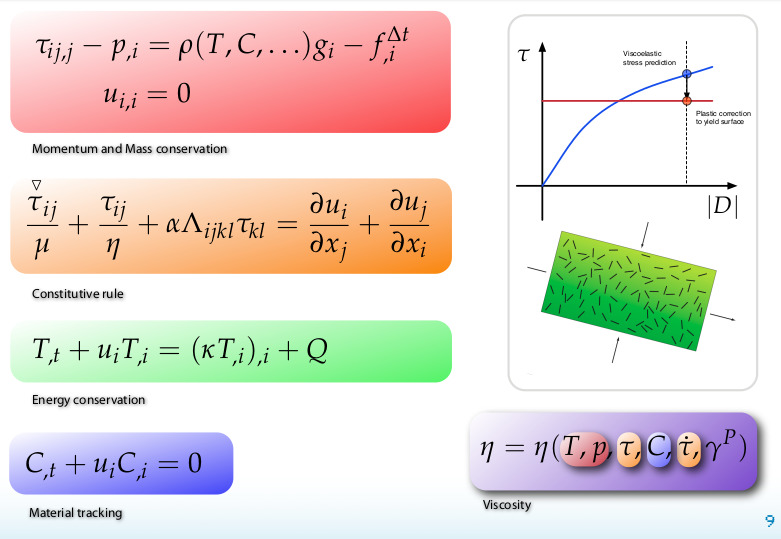
\includegraphics[width=5.5cm]{images/codes/underworld1}
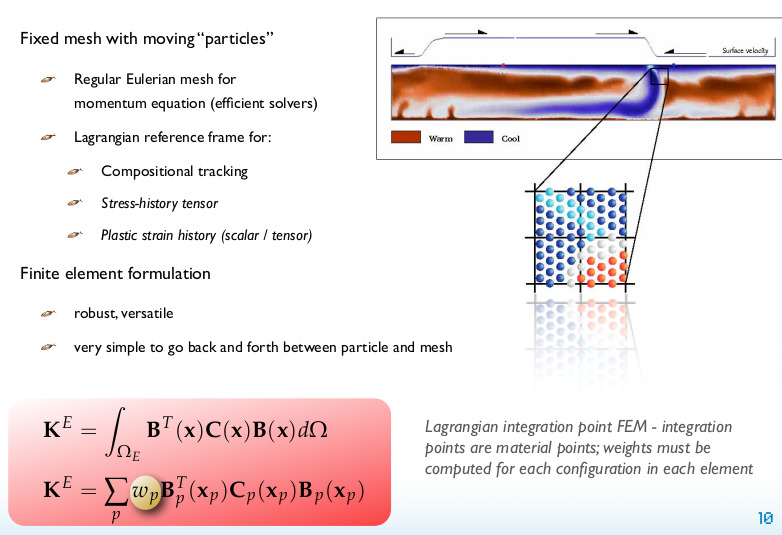
\includegraphics[width=5.5cm]{images/codes/underworld2}
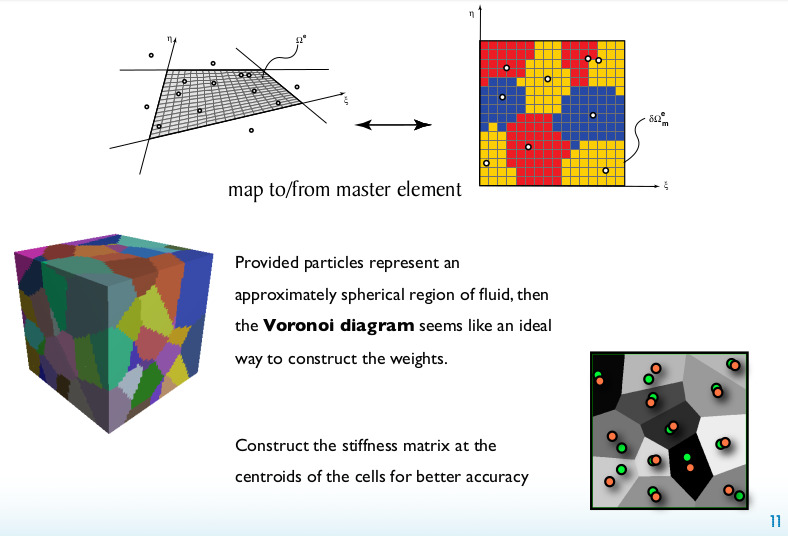
\includegraphics[width=5.5cm]{images/codes/underworld3}\\
{\captionfont Taken from a presentation by L. Moresi}
\end{center}


\begin{scriptsize}
\begin{itemize}
\item[\twothousandsix]       \textcite{stfs06},  \textcite{momu06}
\item[\twothousandseven]     \textcite{moql07},  \textcite{stfs07}, 
                             \textcite{qums07}
\item[\twothousandeight]     \textcite{lemm08},  \textcite{ozrs08}, 
                             \textcite{gotc08},  \textcite{stmt08},
                             \textcite{scsf11}
\item[\twothousandten]       \textcite{casm10},  \textcite{mamb10}, 
                             \textcite{stsf10},  \textcite{stfc10},
                             \textcite{fasm10},  \textcite{cazf10}
\item[\twothousandeleven]    \textcite{memm11},  \textcite{cafz11}
\item[\twothousandtwelve]    \textcite{cafa12}
\item[\twothousandthirteen]  \textcite{bemm12},  \textcite{scmo13}, 
                             \textcite{faca13},  \textcite{care13}, 
                             \textcite{coml13}
\item[\twothousandfourteen]  \textcite{famc14},  \textcite{shjm14}
\item[\twothousandfifteen]   \textcite{quxm15},  \textcite{bemm15}, 
                             \textcite{scsp15},  \textcite{shmj15}, 
                             \textcite{carr15}
\item[\twothousandsixteen]   \textcite{shmv16},  \textcite{onlw16}, 
                             \textcite{kicf16}
\item[\twothousandseventeen] \textcite{bems17},  \textcite{kicf17}, 
                             \textcite{sche17},  \textcite{wakc17}
\item[\twothousandeighteen]  \textcite{memm18},  \textcite{yamz18}, 
                             \textcite{bemc18},  \textcite{mord18}
\item[\twothousandnineteen]  \textcite{samo19},  \textcite{yamg19}, 
                             \textcite{canc19},  \textcite{cakc19},
                             \textcite{sams19b}, \textcite{bore19}
\item[\twothousandtwenty]    \textcite{magm20},  \textcite{sams20}, 
                             \textcite{ghbm20},  \textcite{canc20},
                             \textcite{gumc20},  \textcite{sche20}
\item[\twothousandtwentyone] \textcite{kotr21},  \textcite{qizx21},
                             \textcite{stsc21},  \textcite{zhzl21},
                             \textcite{xiwk21}

\end{itemize}
\end{scriptsize}

%------------------------------------------------------------------------------
\item {\codefont VEMAN}
%------------------------------------------------------------------------------

\begin{scriptsize}
\textcite{bepo10}
\end{scriptsize}

\end{itemize}
